\PassOptionsToPackage{table}{xcolor}
\documentclass{beamer}
\usetheme{default}
\usepackage{color}
\usepackage[color,matrix,arrow]{xypic}
\usepackage{tikz}
\usepackage{tikz-dependency}
\usepackage{tikz-qtree}
\usepackage{tkz-graph}
\usepackage{listings}
\usepackage{caption}
\captionsetup[table]{labelsep=space,labelformat=empty,labelsep=none}
\usetikzlibrary{arrows,positioning}



\title{\color{red}Model introspection}
\subtitle{\emph{Vivisect}}
\date{}

\begin{document}

\makeatletter
\define@key{beamerframe}{wide}[20pt]{
  \def\beamer@cramped{\itemsep #1\topsep0.5pt\relax}}
\makeatother


\setbeamertemplate{frametitle}[default][center]
\centering

\begin{frame}
\titlepage
\end{frame}


\lstdefinestyle{mypython}{
  frame=single,
  language=Python,
  basicstyle=\footnotesize,
  keywordstyle=\bfseries\color{green!40!black},
  commentstyle=\color{orange},
  identifierstyle=\color{blue},
  stringstyle=\color{orange},
  captionpos=b,
  columns=fullflexible,
}
\renewcommand\lstlistingname{}
\renewcommand\thelstlisting{}
\lstset{style=mypython}


\begin{frame}[wide]
  \frametitle{Goals (in parallel with others on inspection team)}
  \pause
  \begin{block}{}
    \begin{itemize}
    \item Inspect model operations in a general, uniform way
    \item Minimal disruption to research patterns
    \item Support the major DNN toolkits
    \end{itemize}
  \end{block}
\end{frame}

\begin{frame}
\frametitle{Current approach from end-user's perspective}
\end{frame}


\begin{frame}[fragile]
  \frametitle{Current approach from end-user's perspective}  
  \begin{lstlisting}[caption={Simple training code}]
import mxnet
 
 
# initialization...
 
model = MyModel(layer_sizes, ...)
 
 
 
for epoch in range(num_epochs):
    model.fit(data)
 
 
# save...
\end{lstlisting}

\end{frame}


\begin{frame}[fragile]
  \frametitle{Current approach from end-user's perspective}
\begin{lstlisting}[caption={Add four lines}]
import mxnet
from vivisect import probe             <1>
 
# initialization...
 
model = MyModel(layer_sizes, ...)
model._vivisect = {"epoch" : 1}    <2>
probe(model, host, port)               <3>
 
for epoch in range(num_epochs):
    model.fit(data)
    model._vivisect["epoch"] += 1  <4>
 
# save...
\end{lstlisting}

\end{frame}


\begin{frame}[fragile]
  \frametitle{Current approach from end-user's perspective}
\begin{lstlisting}[caption={Works for PyTorch and Tensorflow, too}]
import mxnet <--
from vivisect import probe
 
# initialization...
 
model = MyModel(layer_sizes, ...) <--
model._vivisect = {"epoch" : 1}
probe(model, host, port)
 
for epoch in range(num_epochs):
    model.fit(data)
    model._vivisect["epoch"] += 1
 
# save...
\end{lstlisting}
\end{frame}


\begin{frame}[fragile]
  \frametitle{Current approach from end-user's perspective}
\begin{lstlisting}[caption={Import one function}]
import mxnet
from vivisect import probe <--
 
# initialization...
 
model = MyModel(layer_sizes, ...)
model._vivisect = {"epoch" : 1}
probe(model, host, port) <--
 
for epoch in range(num_epochs):
    model.fit(data)
    model._vivisect["epoch"] += 1
 
# save...
\end{lstlisting}
\end{frame}


\begin{frame}[fragile]
  \frametitle{Current approach from end-user's perspective}
\begin{lstlisting}[caption={Arbitrary metadata for downstream}]
import mxnet
from vivisect import probe
 
# initialization...
 
model = MyModel(layer_sizes, ...)
model._vivisect = {"epoch" : 1} <--
probe(model, host, port)
 
for epoch in range(num_epochs):
    model.fit(data)
    model._vivisect["epoch"] += 1 <--
 
# save...
\end{lstlisting}
\end{frame}


\begin{frame}
  \centering
  \frametitle{Example metric plot}
  \includegraphics[height=.7\textheight]{example.png}\\
  Sum of activations (red=LSTM cell, blue=fully-connected)
\end{frame}


\begin{frame}
  \frametitle{``Probe'' attaches callbacks to operations' forward()}
  \pause
  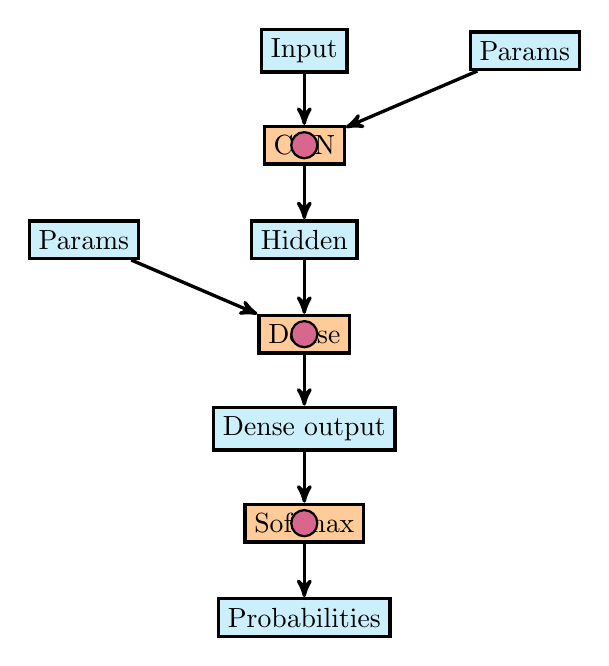
\begin{tikzpicture}  
  \begin{scope}[xshift=-7.5cm,yshift=-5cm,very thick,
		node distance=1.2cm,on grid,>=stealth',
		block/.style={rectangle,draw,fill=cyan!20},
                tr/.style={circle,thick,draw,fill=purple!60},
		comp/.style={rectangle,draw,fill=orange!40}]
    \node [block] (pr)					{Probabilities};
    \node [comp] (sm) [above=of pr]{Softmax} edge [->] (pr);
    \node [block] (fco) [above=of sm] {Dense output} edge [->] (sm);
    \node [comp] (fc) [above=of fco] {Dense} edge [->] (fco);
    \node [block] (cnno) [above=of fc]{Hidden} edge [->] (fc);
    \node [comp] (cnn) [above=of cnno] {CNN} edge [->] (cnno);
    \node [block] (in) [above=of cnn] {Input} edge [->] (cnn);
    \node [block] (parama) [left=of in,xshift=4cm] {Params} edge [->] (cnn);
    \node [block] (paramb) [right=of cnno,xshift=-4cm] {Params} edge [->] (fc);
    \only<3>{
      \node [tr] at (fc.center) {};
      \node [tr] at (cnn.center) {};
      \node [tr] at (sm.center) {};
    }
   \end{scope}
\end{tikzpicture}
\end{frame}


\begin{frame}[fragile]
  \frametitle{Controlling what gets processed and when}
  \begin{lstlisting}[basicstyle=\tiny,columns=fullflexible,otherkeywords={[numpy.array], Operation, Model}]
    probe(m : Model, host : str, port : int, which=lambda x : True, when=lambda x : True) -> None

    
    def example_which(op : Operation):
        return ("RNN" in op._vivisect["name"])

    
    def example_when(m : Model, op : Operation, i : [numpy.array], o : [numpy.array]):
        return (m._vivisect["epoch"] % 10 == 0)

    
    probe(model, host, port, example_which, example_when)
  \end{lstlisting}
  \pause
  \begin{alert}{}
    {Based on this, client code ships an operation's inputs and outputs to the Vivisect server}
    \end{alert}
\end{frame}

\define{\servercolor}{red}
\define{\codecolor}{cyan}
\define{\browsercolor}{brown}

\begin{frame}[fragile]
  \frametitle{Data flow}
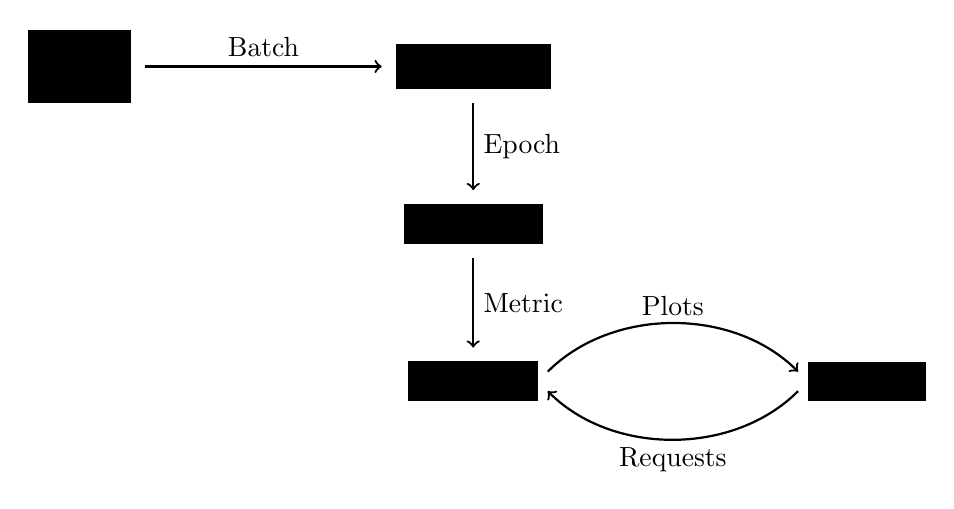
\begin{tikzpicture}[node distance=1cm, auto,
  ]

  \node at (-5, 10) [rectangle, draw=black, thick, fill=\codecolor, text width=3em] (client) { Client code };

  \node at (0, 10) [rectangle, draw=black, thick, fill=\servercolor] (aggregator) { Aggregator };
  \path[->, shorten >=5pt, thick, shorten <=5pt] (client) edge node {Batch} (aggregator);
  
  \node at (0, 8) [rectangle, draw=black, thick, fill=\servercolor] (evaluator) { Evaluator };
  \path[->, shorten >=5pt, thick, shorten <=5pt] (aggregator) edge node {Epoch} (evaluator);
  
  \node at (0, 6) [rectangle, draw=black, thick, fill=\servercolor] (frontend) { Frontend };
  \path[->, shorten >=5pt, thick, shorten <=5pt] (evaluator) edge node {Metric} (frontend);
  
  \node at (5, 6) [rectangle, draw=black, thick, fill=\browsercolor] (browser) { Browser };
  \path[->, bend left=45, thick, shorten >=5pt, shorten <=5pt] (frontend.east) edge node {Plots} (browser.west);
  \path[->, bend left=45, thick, shorten >=5pt, shorten <=5pt] (browser.west) edge node {Requests} (frontend.east);  
  
\end{tikzpicture}
\end{frame}


\begin{frame}[fragile,wide]
  \frametitle{Three metric types}
  \begin{lstlisting}[basicstyle=\large,columns=fullflexible,otherkeywords={[numpy.array]}]
    metric(values : [numpy.array], metadata : dict) -> float
  \end{lstlisting}
  \begin{block}{}
  \begin{itemize}
  \item Intrinsic (magnitude, variance, entropy\ldots)
  \item Supervised (accuracy/fscore from classification, tagging\ldots)
  \item Unsupervised (mutual information from clusterings)
  \end{itemize}
  \end{block}
\end{frame}


\begin{frame}
  \centering
  \frametitle{And browsing to \url{localhost:8080/MODEL/METRIC}\ldots}
  \includegraphics[height=.7\textheight]{example.png}
\end{frame}


\begin{frame}
  
  \begin{block}{Current state:}
    \begin{itemize}
    \item \url{www.github.com/hltcoe/vivisect}
    \item Core structure is working end-to-end
    \item PyTorch and MXNet Gluon are best-supported
    \end{itemize}
  \end{block}
  
  
  \begin{block}{Plans for this month:}
    \begin{itemize}
    \item Implementing lots of metrics
    \item Running on our Sockeye/OpenNMT models
    \end{itemize}
  \end{block}

  \begin{block}{and beyond:}
    \begin{itemize}
    \item Lots of helper functions (which, when) and refactoring
    \item Feature parity with PyTorch (particularly for TF)
    \end{itemize}
  \end{block}
  
\end{frame}

\end{document}
